In this experiment, we varied the message sizes.

\begin{figure*}[!htbp]
        \centering
        \begin{subfigure}[b]{0.32\textwidth}
                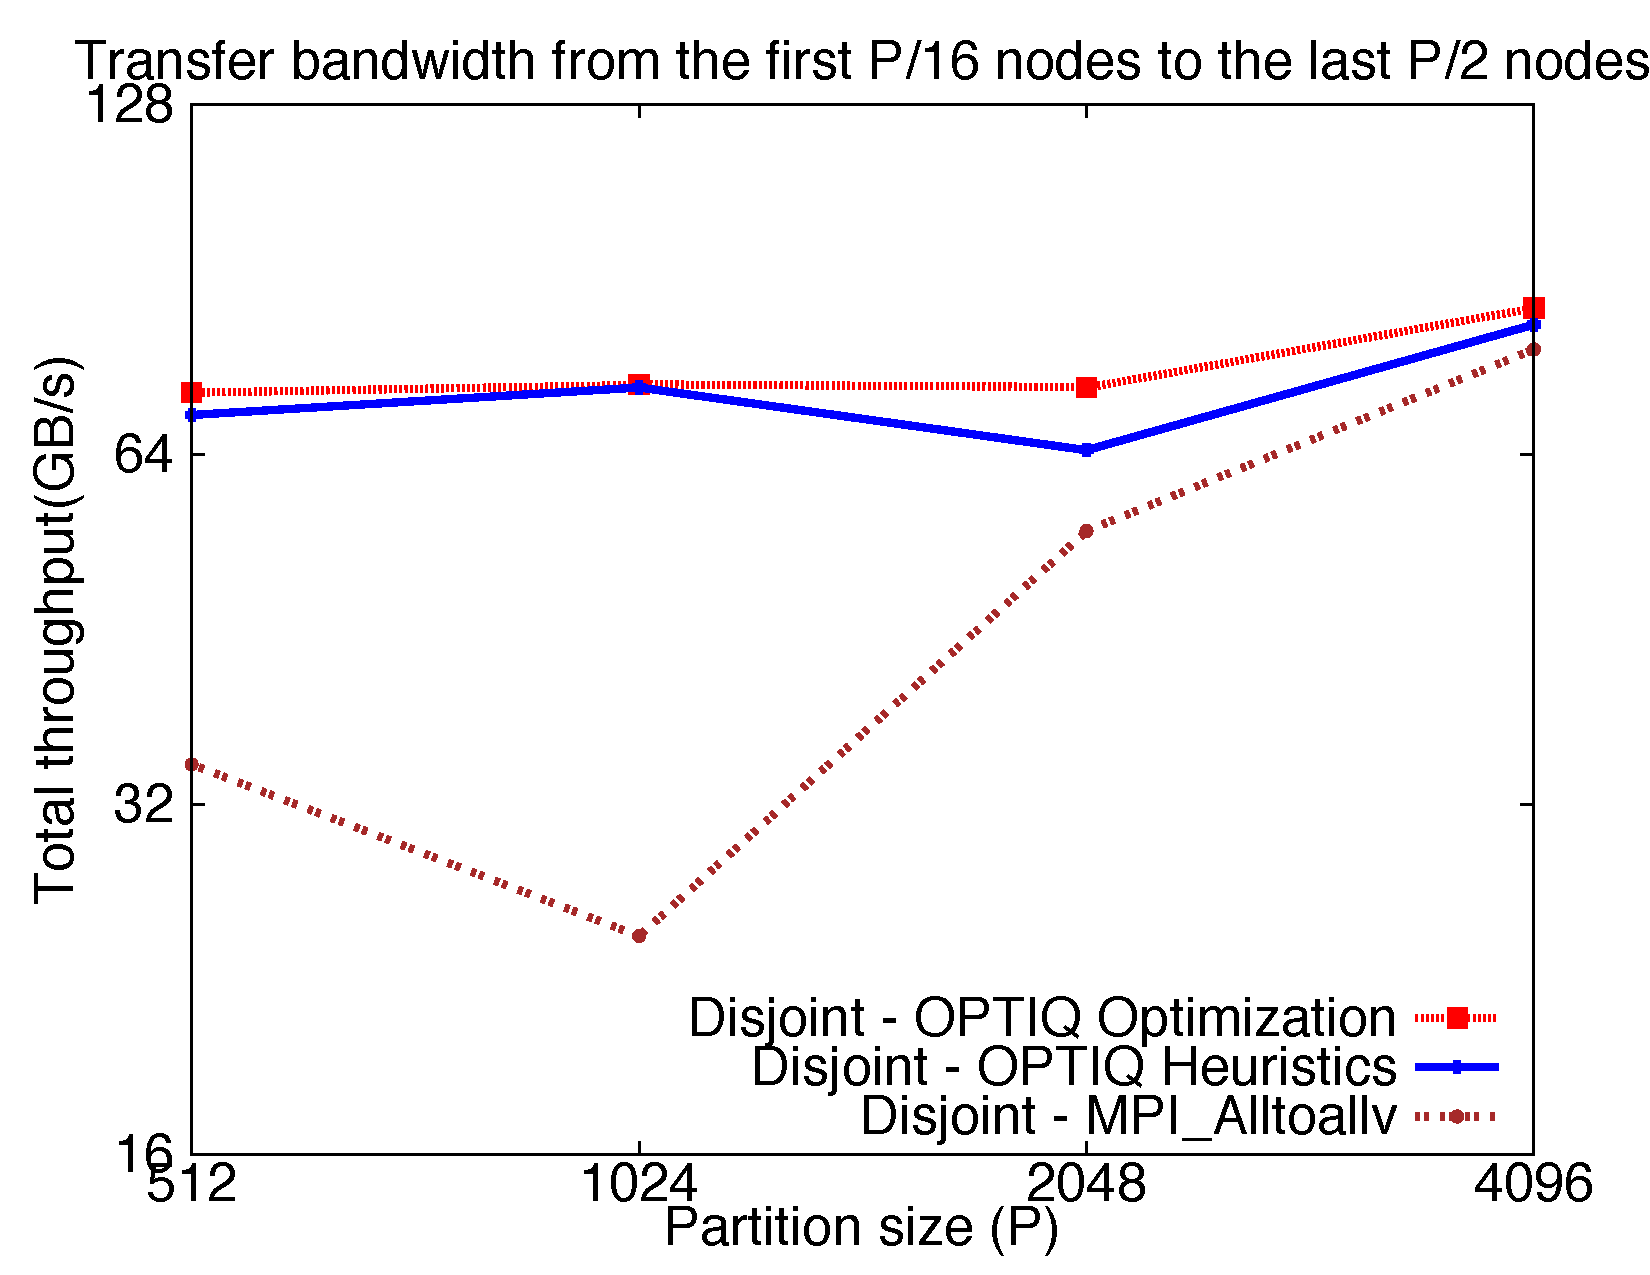
\includegraphics[width=\textwidth]{figures/constantr_disjoint_msg.pdf}
                \caption{Disjoint}
                \label{fig:constantr_disjoint_msg}
        \end{subfigure}%
        ~ %add desired spacing between images, e. g. ~, \quad, \qquad, \hfill etc.
          %(or a blank line to force the subfigure onto a new line)
        \begin{subfigure}[b]{0.32\textwidth}
                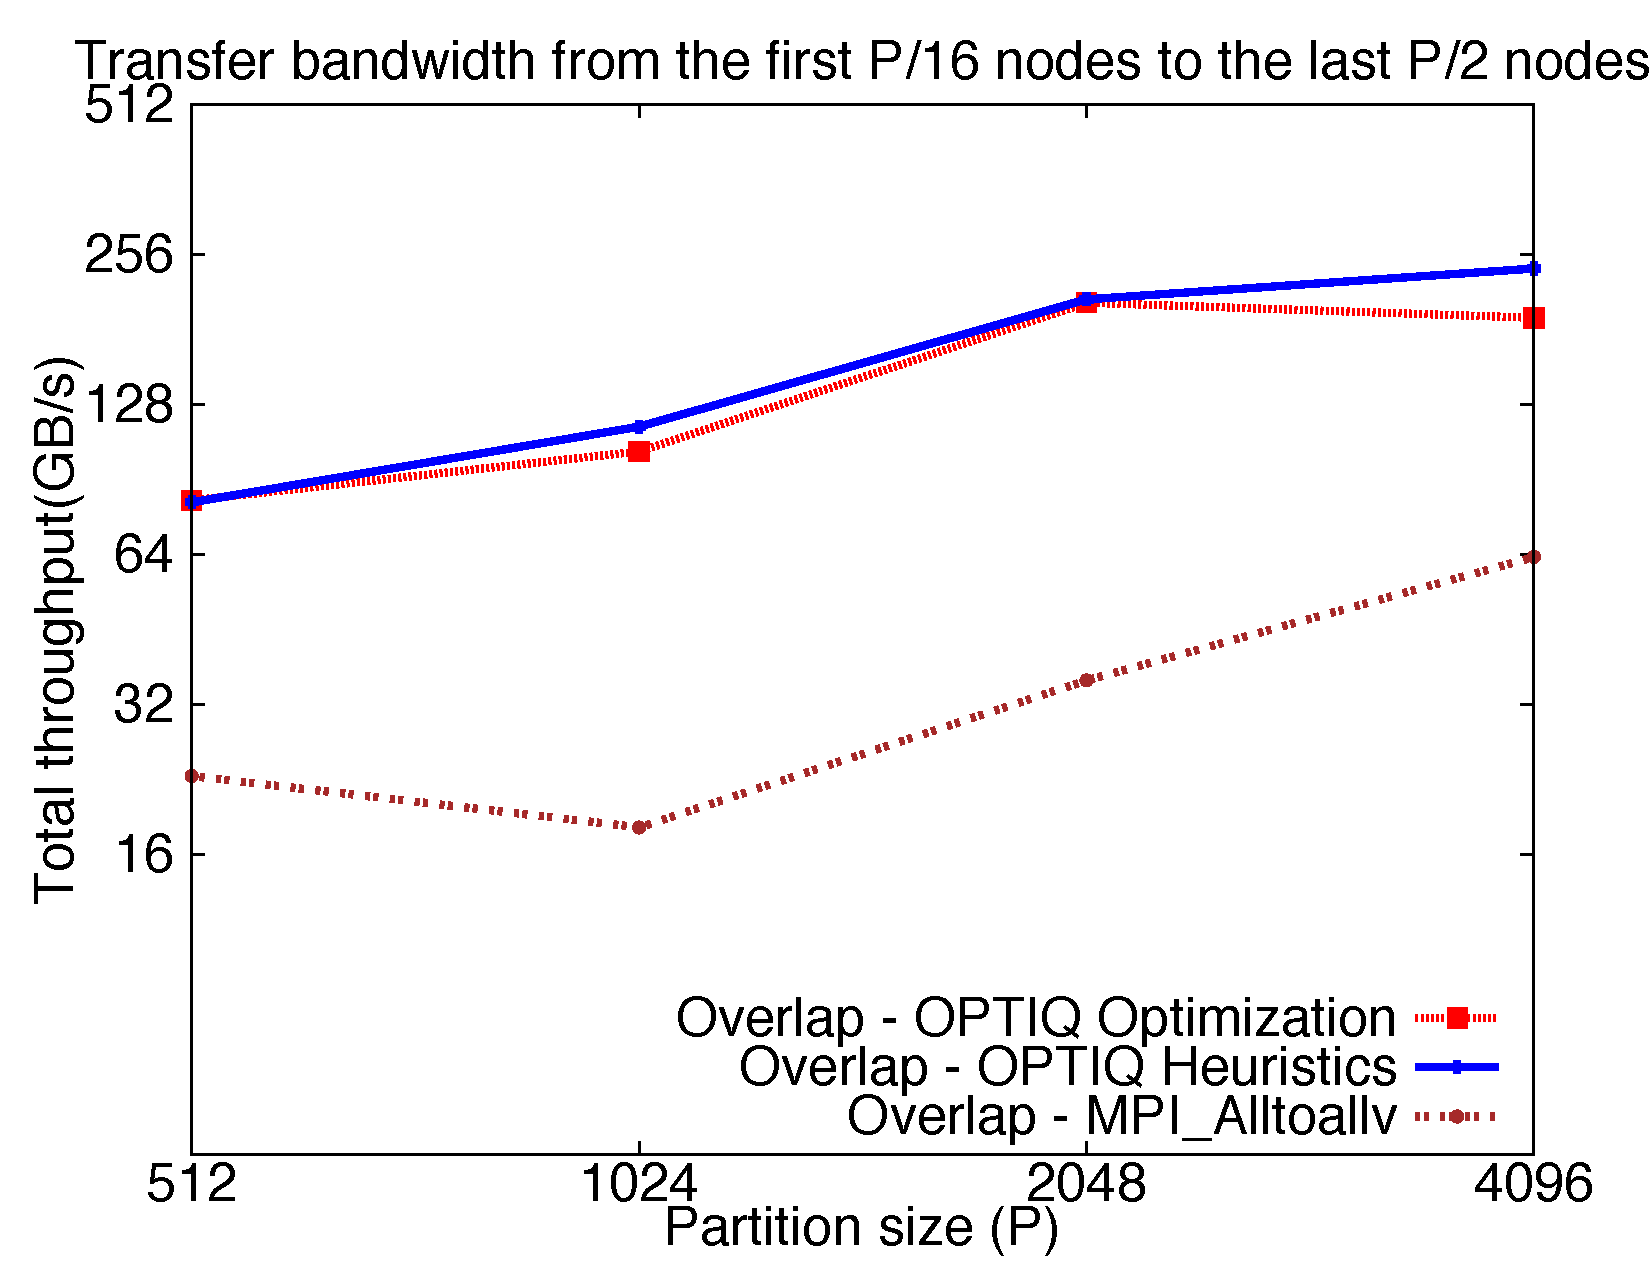
\includegraphics[width=\textwidth]{figures/constantr_overlap_msg.pdf}
                \caption{Overlap}
                \label{fig:constantr_overlap_msg}
        \end{subfigure}
        ~ %add desired spacing between images, e. g. ~, \quad, \qquad, \hfill etc.
          %(or a blank line to force the subfigure onto a new line)
        \begin{subfigure}[b]{0.32\textwidth}
                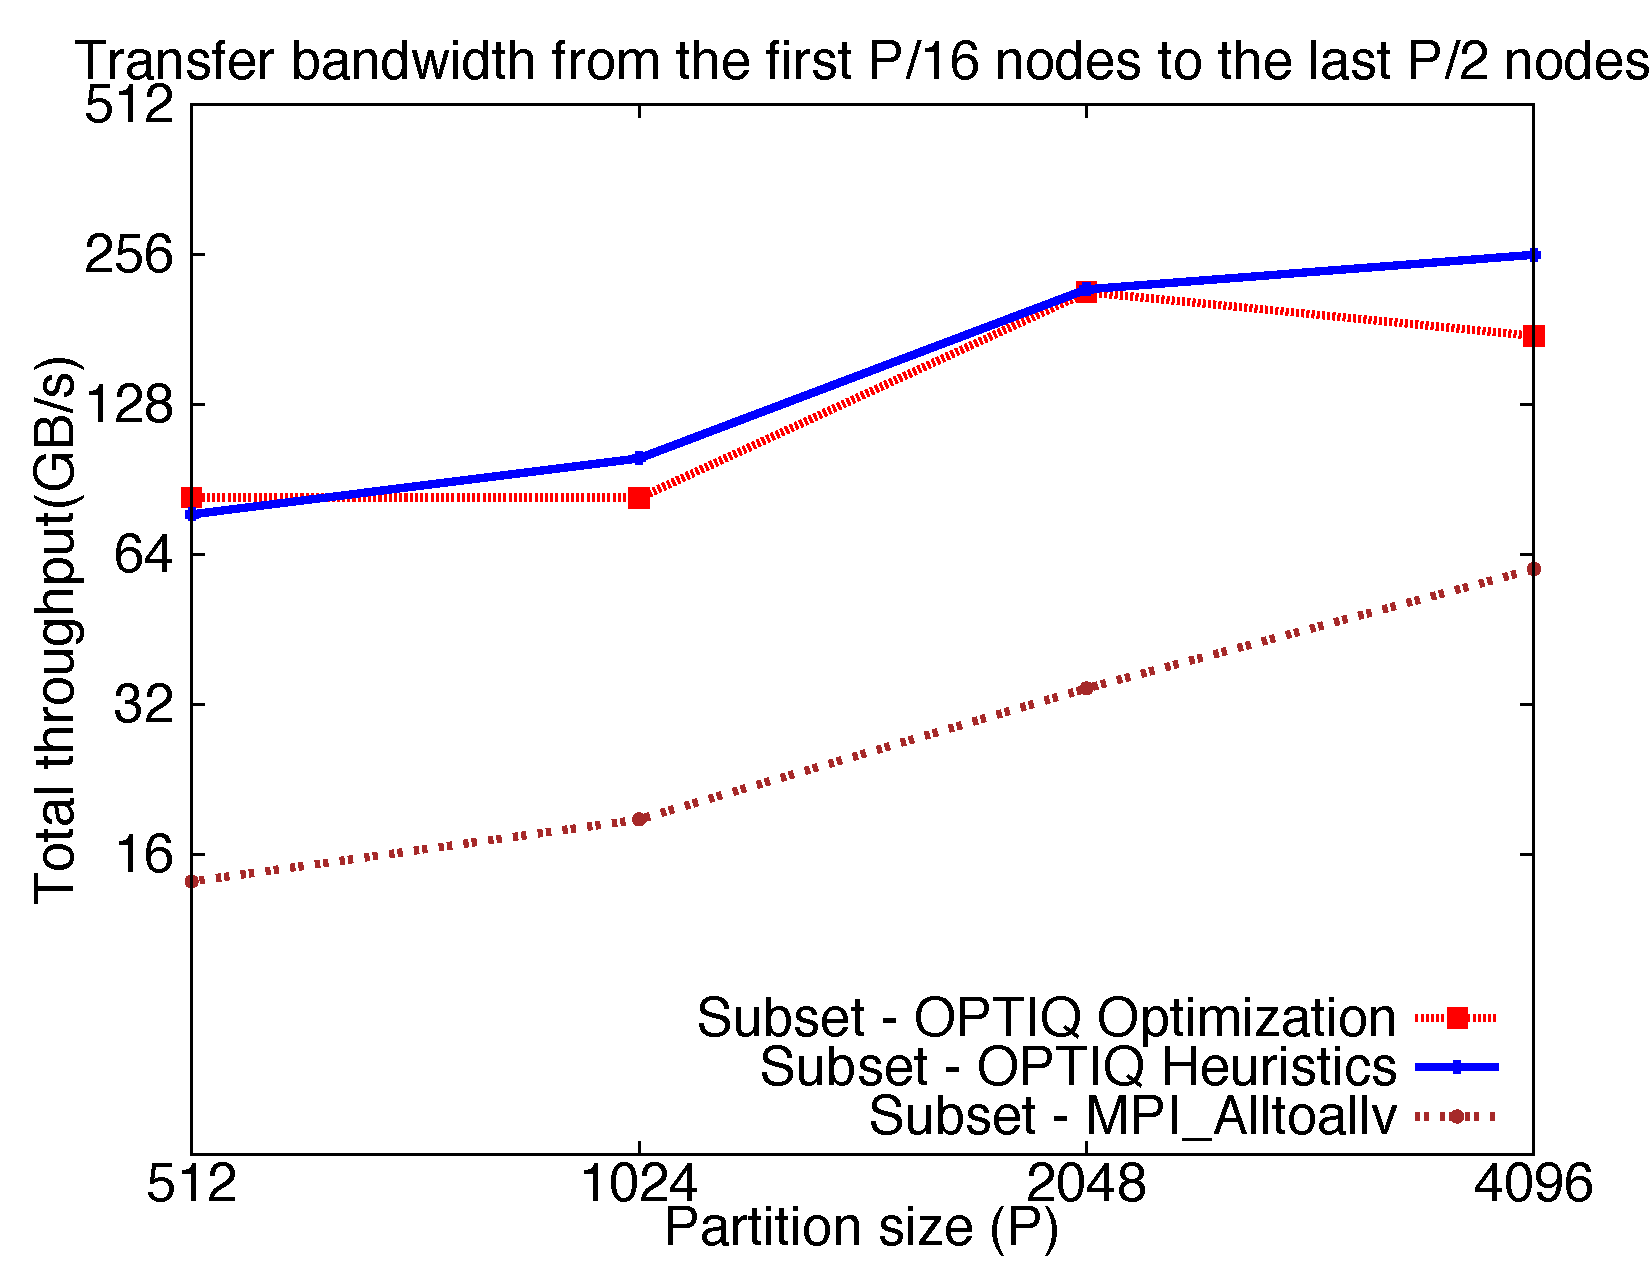
\includegraphics[width=\textwidth]{figures/constantr_subset_msg.pdf}
                \caption{Subset}
                \label{fig:constantr_subset_msg}
        \end{subfigure}
        \caption{Varying the number of sources and destinations and total number of nodes with constant ratio}
        \label{fig:constantr_msg}
\end{figure*}
